\noindent
\paragraph{1 Einführung}\mbox{}\\
\paragraph{1.1 Gleitkommaarithmetik}\mbox{}\\
\begin{itemize}
	\item Rechentechnik auf Maschinen
	\item Fehlerhaft gemäss Konstruktion $\rightarrowtail$ Ungenauigkeiten
\end{itemize}
\paragraph{Darstellung z.B. von $\frac{1}{3}:$}\mbox{}\\
\begin{enumerate}
	\item Konversion in Dezimalzahl mit fixen Anzahl Stellen und verschiebbarem Komma.\linebreak
          exat: $x = \frac{1}{3} = 0.\overline{3} = 0.3333.....$\linebreak
          10-er Gleitkommazahl: $\underbrace{3.333...3}_\text{fixe Anzahl Stellen (16)}\cdot 10^{-1}$\linebreak
          $\rightarrow$ Verlust durch runden an Stelle 16.
    \item Konversion in 2er-Gleitkommazahl \linebreak
          $\rightarrow$ weiteren Verlust.
\end{enumerate}
\paragraph{Hauptproblem: Auslöschung}\mbox{}\\
\begin{itemize}
	\item $
        \begin{rcases}
            \text{$x = 7.341.598.277$} \\
            \text{$y = 7.341.598.253$}
        \end{rcases}
        \rightarrow$ 10 Stellen bekannt
    \item $z = x-y = 0.000.000.024 \rightarrow$ 2 Stellen bekannt \linebreak
                   $\rightarrow 2.4\cdot 10^{-8}$
\end{itemize}
\vspace{1mm}

\paragraph{1.2 Fixpunkt-Iteration}\mbox{}\\
\paragraph{1.2.1 Rekursiv definierte Folgen}\mbox{}\\
\begin{itemize}
	\item Eine Folge kann rekursiv definiert werden durch
	\item S1: Startwert festlegen: $a_0 \in \mathbb{R}$
	\item S2: Rekursion $a_{n+1} = f(a_n)$ für $n \in \mathbb{N}$
	\item Def (Fixpunkt): \linebreak
          Sei $f: \mathbb{R} \rightarrow \mathbb{R}$ eine Funktion, dann heissen die Lösungen der Gleichung\linebreak
          $x = f(x)$ Fixpunkte von f.
    \item Beispiele:
    \item $f(x) = sin(x) \rightarrow$ Fixpunt für $x = 0$.
    \item $f(x) = \frac{1}{x} \rightarrow$ Fixpunkte $\{ -1,1 \}$
\end{itemize}

\paragraph{Satz Existenz von Fixpunkten}\mbox{}\\
\begin{itemize}
	\item Sei $I = \lbrack x_0, x_E \rbrack$ ein Intervall und $f: I \rightarrow I$ stetig (keine Lücken oder Sprünge, etc...), dann hat f mindestens einen Fixpunkt in I.
\end{itemize}


\paragraph{Beweis: graphisch}\mbox{}\\
\noindent
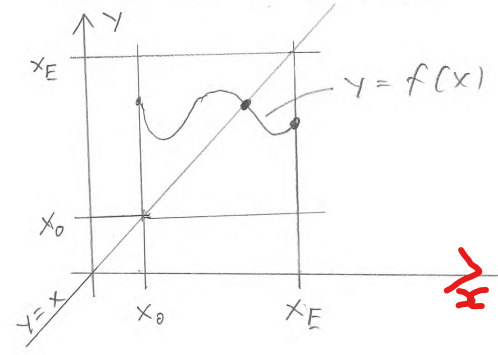
\includegraphics[width=\columnwidth]{./images/beweis_fixpunkt.png}
